\documentclass{deliverablereport}


\usepackage[style=alphabetic,backend=biber]{biblatex}
\addbibresource{../../lib/kbibs/kwarc.bib}
\addbibresource{../../lib/deliverables.bib}
\addbibresource{rest.bib}
% temporary fix due to http://tex.stackexchange.com/questions/311426/bibliography-error-use-of-blxbblverbaddi-doesnt-match-its-definition-ve
\makeatletter\def\blx@maxline{77}\makeatother

% TIkZ magic
\usepackage{tikz,standalone}
\usetikzlibrary{backgrounds,shapes,fit,shadows}
\makeatletter%%%%%%%%%%%%%%%%%%%%%%%%%%%%%%%%%%%%%%%%%%%%%%%%%%%%%%%%%%%%%%%%%
% A TIKZ library for MMT Theory Graphs
% copyright 2014 Michael Kohlhase; Released under the LPPL
%%%%%%%%%%%%%%%%%%%%%%%%%%%%%%%%%%%%%%%%%%%%%%%%%%%%%%%%%%%%%%%%%
%
% this library provides some standardized node and arrow styles for formatting MMT graph
% diagrams in tikz. The advantage is that we can classify the arrows and nodes
% symbolically and with the styles in this library achieve a uniform look that helps
% readability. 
%
%%%%%%%%%%%%%%%%%%%%%%%%%%%%%%%%%%%%%%%%%%%%%%%%%%%%%%%%%%%%%%%%%

%%% 1. Theories
% a generic theory
\def\outerthysep{.3mm}
\def\innerthysep{.5mm}
\tikzstyle{thy}=[draw,outer sep=\outerthysep,rounded corners,inner sep=\innerthysep]
% a primitive theory
\tikzstyle{primthy}=[thy,double]
% a theory graph 
\tikzstyle{thygraph}=[draw,outer sep=1mm,rounded corners,dashed]

%%% 2. Arrows 
%%% 2.1. Arrowtips (only internal)
\usetikzlibrary{arrows}
\newcommand{\@mmtarrowtip}{angle 45}
\newcommand{\@mmtreversearrowtip}{angle 45 reversed}
\newcommand{\@mmtarrowtipepi}{triangle 45}
\newcommand{\@mmtarrowtipmonoright}{right hook}
\newcommand{\@mmtarrowtipmonoleft}{left hook}
\newcommand{\@mmtarrowtippartial}{right to}
\newcommand{\@mmtarrowtippartialleft}{left to}
\newcommand{\@mmtreversearrowtippartial}{right to reversed}
\newcommand{\@mmtreversearrowtippartialleft}{left to reversed}

%%% 2.2 the arrow sstyles in graphs
\usetikzlibrary{decorations,decorations.pathmorphing,decorations.markings}
% any morphism 
\tikzstyle{morph}=[-\@mmtarrowtip,thick] 
\tikzstyle{mapsto}=[|-\@mmtarrowtip] %| any morphism 
% structures
\tikzstyle{struct}=[-\@mmtarrowtip,thick]
% inclusions: regular, partial, and left variants
\tikzstyle{include}=[\@mmtarrowtipmonoright-\@mmtarrowtip,thick]
\tikzstyle{revinclude}=[\@mmtarrowtip-\@mmtarrowtipmonoright,thick]
\tikzstyle{pinclude}=[\@mmtarrowtipmonoright-\@mmtarrowtippartial,thick]
\tikzstyle{includeleft}=[\@mmtarrowtipmonoleft-\@mmtarrowtip,thick]
\tikzstyle{pincludeleft}=[\@mmtarrowtipmonoleft-\@mmtarrowtippartialleft,thick]
% views: regular, mono, partial, and left variants
\tikzstyle{preview}=[decorate,
                                decoration={coil,aspect=0,amplitude=1pt,
                                                    segment length=6pt,
                                                    pre=lineto,pre length=3pt,
                                                    post=lineto,post length=5pt},
                                thick]
\tikzstyle{view}=[preview,-\@mmtarrowtip]
\tikzstyle{mview}=[preview,\@mmtarrowtipmonoright-\@mmtarrowtip]
\tikzstyle{pview}=[preview,-\@mmtarrowtippartial]
\tikzstyle{pmview}=[preview,\@mmtarrowtipmonoright-\@mmtarrowtippartial]
\tikzstyle{viewleft}=[preview,-\@mmtarrowtip]
\tikzstyle{mviewleft}=[preview,\@mmtarrowtipmonoleft-\@mmtarrowtip]
\tikzstyle{pviewleft}=[preview,-\@mmtarrowtippartialleft]
\tikzstyle{pmviewleft}=[preview,\@mmtarrowtipmonoleft-\@mmtarrowtippartialleft]
\tikzstyle{adoption}=[preview,thin,double,-\@mmtarrowtip]
% biviews: regular, partial, and left variants
\tikzstyle{biview}=[preview,\@mmtarrowtip-\@mmtarrowtip]
\tikzstyle{pbiview}=[preview,\@mmtreversearrowtippartial-\@mmtarrowtippartial]
\tikzstyle{pbiviewleft}=[preview,\@mmtreversearrowtippartialleft-\@mmtarrowtippartialleft]
% defining views (experimental)
\tikzstyle{defview}=[preview,densely dotted,-\@mmtarrowtip]
% meta-theory inclusion
\tikzstyle{meta}=[dotted,-\@mmtarrowtip,thick]
% conservative extensions (abbreviation)
\tikzstyle{conservative}=[hooks-\@mmtarrowtip,double] 
% conservative development
\tikzstyle{conservdev}=[hooks-\@mmtarrowtip,dashed,double] 

% antimorphisms as striktthroughs
\tikzset{anti/.style={
    decoration={markings, mark=between positions 0.2 and 0.8 step 4mm with {
        \draw [thick,-] ++ (-3pt,-3pt) -- (3pt,3pt);}},
    postaction={decorate}}}

% parallel markup
\tikzstyle{parallel}=[\@mmtarrowtip-\@mmtarrowtip,dashed]

%%%% 3. Realms 
\tikzstyle{prerealm}=[draw=blue!40,rectangle,rounded corners,inner sep=10pt,inner ysep=20pt]
\tikzstyle{realm}=[prerealm,fill=gray!4]
\tikzstyle{pillar}=[prerealm,fill=gray!10]

%%% 4. convenience macros
%%% 4.1 the \mmtthy macro takes three arguments, name, decl, axioms and makes a 
% table-like structure
\newcommand\mmtthy[3]{\def\@second{#2}\def\@third{#3}%
\begin{array}{l}\textsf{#1}%
\ifx\@second\@empty\else\\\hline #2\fi%
\ifx\@third\@empty\else\\\hline #3\fi%
\end{array}}
%%% 4.2 the \mmtar takes two arguments, some tikz options, and an arrow style. \nmmtar
% is a variant that also has a name on top.
\newcommand\mmtar[2][]{\raisebox{.5ex}{\tikz[#1]{\draw[#2] (0,0) -- (.6,0);}}}
\newcommand\nmmtar[3][]{\raisebox{.4ex}{\tikz[#1]{\draw[#2] (0,0) --
      node[above]{\ensuremath{\scriptstyle #3}} (.8,0);}}}
%%%% 3.3 Pushout symbols
%%  (after http://tex.stackexchange.com/questions/1144/pushouts-and-pullbacks)
%% \nepushout[<pos>]{<basenode>}{<targetnode>} positions a pushout symbol 
%% (available separately as \pushoutsymb) <pos> of the way between <basenode>
%%  and <targetnode>. 
\usetikzlibrary{calc}
\newcommand\@pushout[4][]{\def\@test{#1}%
\ifx\@test\@empty\def\@@num{.5}\else\def\@@num{#1}\fi%
\begin{scope}[shift=($(#2)!\@@num!(#3)$)]\@nameuse{@#4pushoutsymb}\end{scope}} 
\newcommand\@nepushoutsymb{\draw +(-.2,0) -- +(0,0)  -- +(0,-.2);\fill +(-.1,-.1) circle (.03);}
\newcommand\nepushoutsymb{\tikz{\@nepushoutsymb}}
\newcommand\nepushout[3][]{\@pushout[#1]{#2}{#3}{ne}}

\newcommand\@sepushoutsymb{\draw +(-.2,0) -- +(0,0)  -- +(0,.2);\fill +(-.1,.1) circle (.03);}
\newcommand\sepushoutsymb{\tikz{\@sepushoutsymb}}
\newcommand\sepushout[3][]{\@pushout[#1]{#2}{#3}{se}}

\newcommand\@nwpushoutsymb{\draw +(.2,0) -- +(0,0)  -- +(0,-.2);\fill +(.1,-.1) circle (.03);}
\newcommand\nwpushoutsymb{\tikz{\@nwpushoutsymb}}
\newcommand\nwpushout[3][]{\@pushout[#1]{#2}{#3}{nw}}

\newcommand\@swpushoutsymb{\draw +(.2,0) -- +(0,0)  -- +(0,.2);\fill +(.1,.1) circle (.03);}
\newcommand\swpushoutsymb{\tikz{\@swpushoutsymb}}
\newcommand\swpushout[3][]{\@pushout[#1]{#2}{#3}{sw}}

\newcommand\@npushoutsymb{\draw +(-.1,-.1) -- +(0,0)  -- +(.1,-.1);\fill +(0,-.1) circle (.03);}
\newcommand\npushoutsymb{\tikz{\@npushoutsymb}}
\newcommand\npushout[3][]{\@pushout[#1]{#2}{#3}{n}}

\newcommand\@spushoutsymb{\draw +(-.1,.1) -- +(0,0)  -- +(.1,.1);\fill +(0,.1) circle (.03);}
\newcommand\spushoutsymb{\tikz{\@spushoutsymb}}
\newcommand\spushout[3][]{\@pushout[#1]{#2}{#3}{s}}

\newcommand\@wpushoutsymb{\draw +(-.1,-.1) -- +(0,0)  -- +(-.1,.1);\fill +(-.1,0) circle (.03);}
\newcommand\wpushoutsymb{\tikz{\@wpushoutsymb}}
\newcommand\wpushout[3][]{\@pushout[#1]{#2}{#3}{w}}

\newcommand\@epushoutsymb{\draw +(.1,.1) -- +(0,0)  -- +(.1,-.1);\fill +(.1,0) circle (.03);}
\newcommand\epushoutsymb{\tikz{\@epushoutsymb}}
\newcommand\epushout[3][]{\@pushout[#1]{#2}{#3}{e}}

%%%%%% testing them: 
% \begin{tikzpicture}[scale=1.5]
%   \node (a) at (0,0) {a};
%   \node (b) at (1,0) {b};
%   \node (c) at (1,1) {c};
%   \node (d) at (0,1) {d};
%   \nepushout[.8]{a}c;
%   \nwpushout[.8]{b}d;
%   \sepushout[.8]{d}b;
%   \swpushout[.8]{c}a;
%   \draw (a) -- (b) -- (c) -- (d) -- (a);
%   \node (aa) at (4,0) {a};
%   \node (bb) at (3.5,.5) {b};
%   \node (cc) at (4,1) {c};
%   \node (dd) at (4.5,.5) {d};
%   \draw (aa) -- (bb) -- (cc) -- (dd) -- (aa);
%   \npushout[.8]{aa}{cc};
%   \spushout[.8]{cc}{aa};
%   \wpushout[.8]{bb}{dd};
%   \epushout[.8]{dd}{bb};
% \end{tikzpicture}

%%% Local Variables:
%%% mode: latex
%%% TeX-master: "test"
%%% End:
\makeatother

\usepackage{standalone}
\usepackage[show]{ed}

\usepackage{graphicx}
\usepackage{float}

\usepackage{color}
\definecolor{gray}{rgb}{0.4,0.4,0.4}
\definecolor{darkblue}{rgb}{0.0,0.0,0.6}
\definecolor{cyan}{rgb}{0.0,0.6,0.6}

\deliverable{dksbases}{design}
\issue{136}
\deliverydate{31/08/2016}
\duedate{31/08/2016 (Month 12)}
\def\pn{OpenDreamKit\xspace}

\author{Michael Kohlhase}
\author{Florian Rabe}
\author{Tom Wiesing}
\address{Jacobs University Bremen}
\author{Paul-Olivier Dehaye}
\address{Z\"urich University}
%\title{-- ??title?? -- }

\usepackage[parfill]{parskip}

% for definitions
\usepackage{amsthm}
\newtheorem{mydef}{Definition}

\begin{document}

\maketitle\vfill

\begin{abstract}
Yet to do
\end{abstract}

\vfill

\newpage\tableofcontents\newpage

\ednote{Write an abstract}
\ednote{Update delivery data}

\section{Introduction}\label{sec:intro}

The goal of the OpenDreamKit project \cite{ODKproposal:on} is to develop a generic Toolkit that will enable Mathematicans (and scientists in general) to build so-called Virtual Research Environments (VREs) that are optimally tailored to specific communitites. These will combine a multitude of different tasks, such as symbolic mathematics, automatic code generation, numerical computation, data bases, post-processing or visualisation. A VRE will provide end-users with a single tool-chain that can be used for most, if not all, of their research.

To be able to build such a toolkit, we will need to combine three different aspects -- Data (D), Knowledge (K) and Systems. Ultimatly we want to create and make use of them using a VRE; we want to model the real world, translate it into a set of mathematical objects and computationally simulate and thereby explore them.

The Data aspect is commonly manifested inside databases as tables or lists of numerical or symbolic data. The systems aspect is reprented by mathematical knowledge systems (MKS), such as GAP, Sage, \dots and others computing on top of this data. The knowledge aspect is in between these two, providing both the basis for the data that is stored inside Databases and the basis for the algorithms implemented inside the software. An illustration with more examples of these aspects can be found in Figure~\ref{fig:thebigpicture}.

\begin{figure}[H]
  \centerline{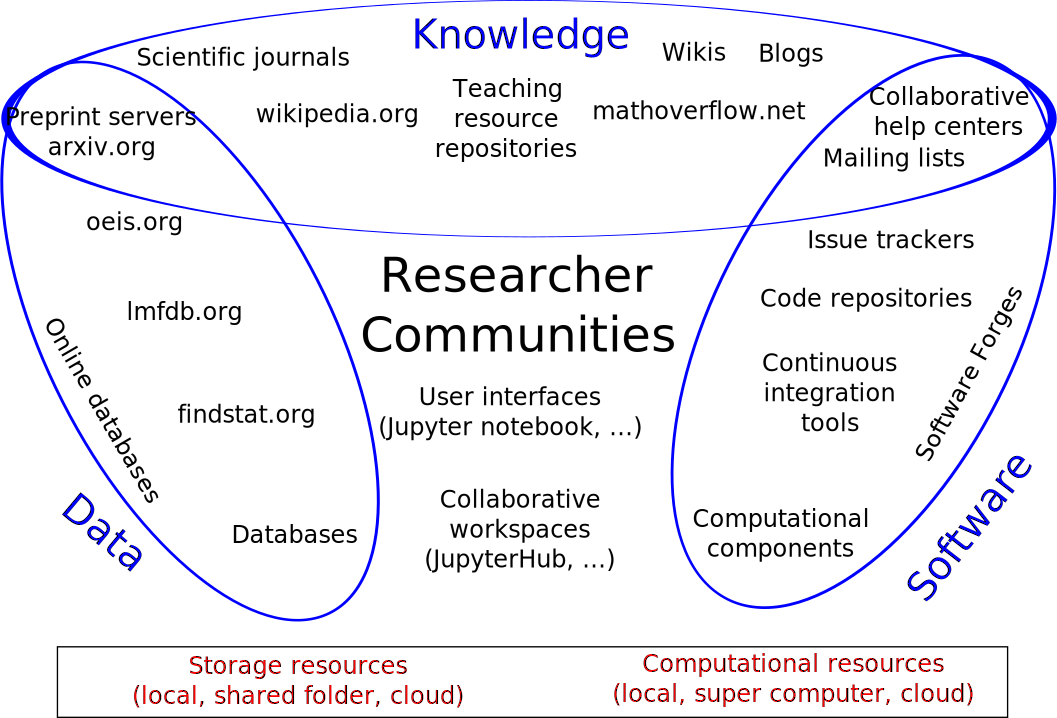
\includegraphics[width=\textwidth]{../../Proposal/Pictures/TheBigPicture.pdf}}
  \caption{Virtual Research Environments for research in pure
    mathematics and applications.}
  \label{fig:thebigpicture}
\end{figure}

To achieve the task of building a VRE with these three aspects we want to use the well-established framework of theory graphs -- which we will briefly explain below in \ref{sec:mmt}. As a basis towards building DKS theories we use the MMT system -- our existing implementation of theory graphs -- which has K(nowledge) theories already. We split the remaining task in two, integrating \textit{systems and knowledge} (Section~\ref{sec:mitm}) and integrating \textit{knowledge and data} (Section~\ref{sec:introfinal}).

\subsection{A Brief Recap of Theory Graphs}\label{sec:mmt}

A theory graph consists of theories and the relations between them. A theory in this sense is a set of declarations -- a set of declared symbols. In addition to the declarations, each theory has a name (which together with its namespace forms the global URI for the theory) and a meta-theory. A meta-theory is commonly the logical framework that is used to model the content of the theory. Each declared symbol has a name and can additionally have a type, a definition and different kinds of meta-data. In each theory these symbols can then be used to form terms that can be used to express more advanced knowledge. Here terms are effectively OpenMath 2.0 \cite{BusCapCar:2oms04} objects -- they mostly consist of literal values, symbols and applications of terms to other terms.

There are two basic kinds of relations between theories: imports and views. An import is a way to declare symbols from one theory in another theory -- to import the symbols from a source theory to a target theory. This can for example be used to extend an existing theory without re-declaring all symbols or to combine two theories. Furthermore the concept of imports allows to modularise knowledge. On top of imports there are also Structures which are imports and additional renamings of the imported symbols. The second type of relation, the view, is a mapping from one theory to another -- a way to ``view'' one theory as another. This mapping allows terms from one theory to be translated into another theory. In the case where terms represent boolean statements or proofs, the mapping given by the view is truth preserving -- \emph{i.e.}~if a statement is true in the source theory, it is be true in the target theory after translation.

Theory graphs are implemented inside the MMT system \cite{RabKoh:WSMSML13}. The system allows for the declaration of theories along with symbols, imports and views. Furthermore it is possible to create terms over these theories and translate them along views. The MMT system also provides a type checker that can be used to type check declarations.

\subsection{Using the Math-In-The-Middle approach to integrate systems}\label{sec:mitm}

When integrating multiple system we are mostly talking about using concrete algorithms (implemented by these systems) to solve a specific computational problem (the knowledge about the problem). To integrate multiple systems woth this knowledge we want to enable users to write down a problem in one system and then solve it in another system. We want to be independent of the implementation of the knowledge -- independent of the systems.

For this we make use of an approach we call Math-In-The-Middle. Here the underlying mathematical knowledge, the ``real math'', is in betweeen (in the ``middle'') of the systems -- hence the name. Each system needs access to this knowledge. As each of them come with their own particularities, they will need some interface to it.

We want to make use of the modular approach to mathematics provided by theory graphs, and in particular MMT as an implementation thereof, to first of all allow us translate mathematical expressions between systems. We define a ``Math In The Middle'' theory as well as interface theories for each system. With the help of MMT and bi-views\footnote{A bi-view is a bidirectional view between two theories} between the interface theories and the central theory, we can translate objects from one system to the other.

\begin{figure}[ht]\centering
  \documentclass{standalone}
\usepackage[mh]{mikoslides}
% this file defines root path local repository
\defpath{MathHub}{/Users/kohlhase/localmh/MathHub}
\mhcurrentrepos{MiKoMH/talks}
\libinput{WApersons}
% we also set the base URI for the LaTeXML transformation
\baseURI[\MathHub{}]{https://mathhub.info/MiKoMH/talks}

\usetikzlibrary{backgrounds,shapes,fit,shadows,mmt}
\begin{document}
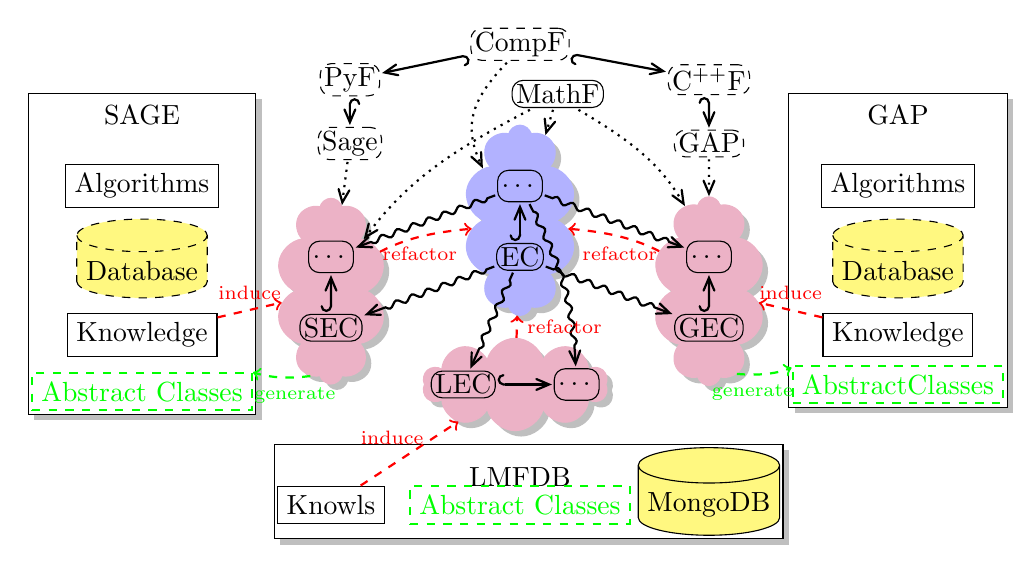
\begin{tikzpicture}[xscale=2.4,yscale=.9]
  \tikzstyle{withshadow}=[draw,drop shadow={opacity=.5},fill=white]
   \tikzstyle{database} = [cylinder,cylinder uses custom fill,
      cylinder body fill=yellow!50,cylinder end fill=yellow!50,
      shape border rotate=90,
      aspect=0.25,draw]
   \tikzstyle{human} = [red,dashed,thick]
   \tikzstyle{machine} = [green,dashed,thick]

\node[thy]  (mf) at (.2,5.3) {MathF};
\node[thy,dashed]  (compf) at (0,6) {CompF};
\node[thy,dashed]  (pf) at (-.9,5.5) {PyF};
\node[thy,dashed]  (cf) at (1,5.5) {C\textsuperscript{++}F};
\node[thy,dashed]  (sf) at (-0.9,4.6) {Sage};
\node[thy,dashed]  (gf) at (1,4.6) {GAP};

\draw[include] (compf) -- (pf);
\draw[includeleft] (compf) -- (cf);
\draw[include] (pf) -- (sf);
\draw[includeleft] (cf) -- (gf);

\node[thy] (kec) at (0,3) {EC};
\node[thy,minimum height=.4cm] (kl) at (0,4) {\ldots};

\node[thy] (sec) at (-1,2) {SEC};
\node[thy,minimum height=.4cm] (sl) at (-1,3) {\ldots};

\node[thy] (gec) at (1,2) {GEC};
\node[thy,minimum height=.4cm] (gl) at (1,3) {\ldots};

\node[thy] (lec) at (-.3,1.2) {LEC};
\node[thy,minimum height=.4cm] (ll) at (.3,1.2) {\ldots};

\node (sc) at (-2,5) {SAGE};
\node[draw] (salg) at (-2,4) {Algorithms};
\node[database,dashed] (sdb) at (-2,2.8) {Database};
\node[draw] (skr) at (-2,1.9) {Knowledge};
\node[draw,machine] (sac) at (-2,1.1) {Abstract Classes};

\node (gc) at (2,5) {GAP};
\node[draw] (galg) at (2,4) {Algorithms};
\node[database,dashed] (gdb) at (2,2.8) {Database};
\node[draw] (gkr) at (2,1.9) {Knowledge};
\node[draw,machine] (gac) at (2,1.2) {AbstractClasses};

\node (lmfdb) at (0,-.1) {LMFDB};
\node[database] (ldb) at (1,-.5) {MongoDB};
\node[draw] (knowls) at (-1,-.5) {Knowls};
\node[draw,machine] (lac) at (0,-.5) {Abstract Classes};

  \begin{pgfonlayer}{background}
    \node[draw,cloud,fit=(sec) (sl),aspect=.4,inner sep=-3pt,withshadow,purple!30] (st) {};
    \node[draw,cloud,fit=(gec) (gl),aspect=.4,inner sep=-4pt,withshadow,purple!30] (gt) {};
    \node[draw,cloud,fit=(kec) (kl),aspect=.4,inner sep=0pt,withshadow,blue!30] (kt) {};
    \node[draw,cloud,fit=(lec) (ll),aspect=3.5,inner sep=-8pt,withshadow,purple!30] (lt) {};
  \end{pgfonlayer}

\begin{pgfonlayer}{background}
  \node[draw,withshadow,fit=(sc) (skr) (sac) (sdb),inner sep=1pt] {};
  \node[draw,withshadow,fit=(gc) (gkr) (gac) (gdb),inner sep=1pt] {};
  \node[draw,withshadow,fit=(lmfdb) (lac) (ldb) (knowls),inner sep=1pt] {};
\end{pgfonlayer}

\draw[view] (kec) -- (sec);
\draw[view] (kec) -- (gec);
\draw[view] (kec) -- (lec);
\draw[include] (kec) -- (kl);
\draw[include] (gec) -- (gl);
\draw[include] (sec) -- (sl);
\draw[include] (lec) -- (ll);
\draw[view] (kl) -- (sl);
\draw[view] (kl) -- (gl);
\draw[view] (kl) to[bend left=5] (ll);

\draw[meta] (mf)  to [bend right=10] (st);
\draw[meta] (sf) -- (st);
\draw[meta] (mf)  to [bend left=10] (gt);
\draw[meta] (gf) -- (gt);
\draw[meta] (mf) -- (kt);
\draw[meta] (compf) to[bend right=15] (kt);

\draw[human,->] (skr) -- node[above]{\scriptsize induce} (st);
\draw[human,->] (gkr) -- node[above]{\scriptsize induce} (gt);
\draw[human,->] (knowls) -- node[left,near end]{\scriptsize induce} (lt);

\draw[machine,->] (gt) to[bend right=30] node[below,near start]{\scriptsize generate} (gac);
\draw[machine,->] (st) to[bend left=30] node[below,near start]{\scriptsize generate} (sac);
\draw[human,->] (st) to[bend left=20] node[below]{\scriptsize refactor} (kt);
\draw[human,->] (gt) to[bend right=20] node[below]{\scriptsize refactor} (kt);
\draw[human,->] (lt) -- node[right]{\scriptsize refactor} (kt);
\end{tikzpicture}
\end{document}
%%% Local Variables: 
%%% mode: latex
%%% TeX-master: t
%%% End: 

  \caption{The MitM paradigm in detail. PyF, C${}^{++}$F and CompF are (basic) foundational theories for \textit{Python}, C${}^{++}$ and a generic computational model. SEC, LEC and GEC are theories for \textit{Sage}, \textit{LMFDB} and \textit{GAP} elliptic curves.}\label{fig:mitm}
\end{figure}

A sketch of the theory graph based on the example of elliptic curves can be found in Figure~\ref{sec:mitm}. We will not go into details here -- we have alread disucssed the approach in \cite{DehKohKon:iop16}. Instead we focus on the second part of the problem, integrating Data with Knowledge.

\subsection{Data-Knowledge Theories as a step towards DKS}\label{sec:introfinal}

The theories currently implemented inside MMT are very good at formalising a variety of knowledge, however are limited when it comes to representing a big amount of data. They are are effectively K(nowledge)-Theories. To build the OpenDreamKit VREs however we need to be able to utilise them for Data and different systems as well. As an initial design step towards this we need to expand the theory graph model with a concept of Data-Knowledge theories -- this is what we will focus on in this report.

In Section~\ref{casestudy}, we will first of all present the different systems that are most relevant to the OpenDreamKit project. Next in Section~\ref{sec:data} we describe in detail our concept of Data-Knowledge theories, and our implementation thereof in Section~\ref{sec:impl}. Continuing in Section~\ref{sec:cases} by showing and explaining which databases we have integrated into our efforts already. Next we show in Section~\ref{sec:querying} how we plan to enable users to query and make further use of DK-theories before finally concluding with a short summary and outlook in Section~\ref{sec:conclusion}.

\section{Report and Case-Study}\label{casestudy}
\ednote{Paul: give a general overview of the results of the case-study}

\section{Data-Knowledge Theories}\label{sec:data}

To work with DK theories, the first thing we need to do is define them.
\begin{mydef}[DK theory]
  A Data-Knowledge (or DK for short) theory is a theory consisting of a potentially infinite set of declarations.
\end{mydef}

But what does this mean? To clarify this, we list a few examples here. The first thing to note is that all K-theories represented inside MMT are DK theories that contain a very limited set of finitely many declarations. However this only part of what is covered by this concept -- it becaomes interesting once we have many more declarations inside a theory, in the sense that we have sufficiently many that we can not keep them all in memory or want to materialise all of them on disk.

Consider the problem of formalising the natural numbers inside a theory. For this we could use a theory with as little as eight declarations -- one for the type of natural numbers, one for the number zero, one for the successor function and one for each of the five Peano axiomes. This defines a DK theory however it is not very practical. We could use terms for each of the natural numnbers, but if we want to write down a number like $365$, we would have to apply the successor function $365$ times. We really want to have one declaration for each natural number, i.e. have each number declared as the successor of the previous one. This is in the spirit of DK theories.

The naive approach to implement this theory does not work -- we would need to hold infitely many declarations in memory. Even if we had infinite memory, this would not be enough -- we would need to materialise all of these definitions in the first place -- we can not just write all of them down. This particular example can be solved by introducing literals -- but that is not the point. It illustrates the basic problem that comes up in many practical situations. We have a very big set of declarations that are generated according to some schema. This can mean that there is an obvious pattern to generate all of them -- like with natural numbers -- or that they are stored in some external database or system. In the database system there is some pattern in how to generate the declarations -- each declaration corresponds to a record inside the database.

LMFDB is a mathematical database that contains a collection of elliptic curves. We can use this to define a DK theory consisting of elliptic curves\footnote{And indeed we have done this. More on what LMFDB is and what exactly we have achieved so far can be found below in Section~\ref{sec:lmfdb}}. We could furthermore extend this theory to not only include elliptic curves, but all objects contained inside LMFDB. Inside this theory, not all declarations will look the same -- they will all be of different types. It should also be noted that this theory is not something one would want to write down manually -- even though there are finitely many declarations. Likely the number of declarations is vastly bigger than what we can hold in main memory at any point.

In practice we will never need to access all of these declarations at once -- in most scenarios we will only need a very small subset of them. A small subset that is big enough to hold in memory. Hence we need some process to load the declarations inside main memory once we need them -- or possibly even create them if they do not yet exist.
\begin{mydef}[Virtual theory]
  A Virtual Theory is an implementation of a DK theory that loads or creates declarations in main memory on demand and unloads them once memory space becomes limited.
\end{mydef}
This adresses the problems we mentioned above. On top of the requirements already defined, we ideally want such an implementation to be invisible to the user -- they should not notice the difference between a K theory and a DK theory that contains on-demand declarations.

While there are many possible implementations for DK theories, here we only concern ourselves with the case where the declaration come from some arbitary external database. On top of retrieving declarations from DK theories, we also want to be able to create new declarations, update existing ones and possibly even delete some. In the case of some underlying database this corresponds perfectly to the CRUD -- Create, Read, Update, Delete -- operations. We can just translate the operations and have the database take care of the implementation details. \ednote{Possibly link to query section here}

\section{Relating Database structure and Mathematical objects}\label{sec:impl}

The first step towards implementing Virtual Theories is to create a theory that retrieves declarations from inside a database. Databases are not commonly optimise for mathematical objects. On the contrary -- databases usually enforce their own schema that does not correspond in any way to the high-level mathematical objects that we want to model. Furthermore the object representations are not in the form of something resembling OpenMath / MMT terms -- usually they are in primitive objects (integers, strings, booleans, etc. ) or in data formats like JSON.

Hence we need to be able to translate between the low-level representations of the objects stored in the database and the underlying mathematical objects (in the form of MMT terms). In most common databases, each record stored usually has multiple fields that each have values. Each field commonly represents one property of the mathematical object. Together the fields and their values are more than enough to uniquely define the mathematical object. The values themselves are usually represented with some physical data type -- for example an integer is stored in the form of a 64-bit integer\ednote{Better example?}. In some of the cases it is trivial to translate the encoded values to the proper values. In other cases, it might not be as trivial as it seems. Take for example a mathematical object defined by some matrix of integers. On one hand it could simply be represented as a list of list of integers. On the other hand the database could use some kind of sparse representation, i.e. store only the non-zero entries. To encompass this setup inside MMT we introduce the concept of codecs.

\begin{mydef}[Codec]
A codec is a triple $(t, f, g)$ where $t$ is a type (represented as a term inside the Math-In-The-Middle Theory), $f$ a mapping from the encoded representations of the type to the intended values of the type and $g$ is a mapping from the actual values of the type to their physical encodings. We call the operation performed by $f$ a decoding and the operation performed by $g$ an encoding of the type $t$.
\end{mydef}

We can use codecs to translate between MMT terms and the database objects. There are two basic ways of creating codecs -- atomic codecs and codec operators. An atomic codec is a codec of a very simple type, for example an encoding of integers as strings. In this case $f$ would be a map from strings consisting of digits\footnote{Technically, there may also be a starting \texttt{"-"} or \texttt{"+"} sign, but the details are not important here. } to integers. This mapping does exactly what you would expect -- it maps the string \texttt{"0"} to 0, the string \texttt{"1"} to 1, etc. $g$ would be an inverse of sorts -- the map from integers to strings that maps 0 to \texttt{"0"}, 1 to \texttt{"1"}, etc. Note that here $g$ is the left inverse of $f$ (in the sense that $g \circ f$ is the identity), but $f \circ g$ not neccessarily. In a general setting we want $g \circ f$ to be the identity for all codecs, however in practive it rarely happens. A good example of this is the problem of precision -- there is no chance of encoding all of the real numbers in a physical (countable, probably even finite) datatype.
The second way of creating codecs is by using codec operators. These take as input an atomic codec and give a codec for a composite type. Take for example the list codec operator. It takes as input a codec for an arbitary type $t$ and gives a codec for the type \texttt{List(t)}.

Inside MMT we can represent the actual values as literals. For this we do not use the representations from the database, but instead values that best represent the true values. We also represent the codecs inside MMT. Each codec can be represented as an MMT term, with each atomic codec  and each codec operator having an associated symbol inside a Codec theory We can use these symbols to represent arbitary codecs, for example a codec for a matrix of integers would be represented by applying the symbol for a matrix codec operator to the symbol for an integer codec. For each codec and codec operator we have an associated Scala class. For atomic codecs, this class implements an \texttt{encode} and \texttt{decode} method (implementing $g$ and $f$ respectively). In the case of Codec operators, it implements a \texttt{build\_codec}\ednote{Correct method name} method -- that takes as input an AtomicCodec and returns an codec for the composite type.

To be able to construct the codec that corresponds to a Term we have also implemented a Coder class\ednote{Different name?}. It starts from a term representing a codec, finds the appropriate atomic codec(s) and codec operator(s) and then uses them to construct a Codec instance. This allows us given a literal value  and a Term representing its type to encode or decode terms in almost arbitary ways.

\subsection{Using Records and Schemas inside MMT}

Codecs only solve half of the problem -- they can only translate values. We still need to represent the records as a whole inside DK theories. For this we introduce a type of records inside MMT. This is just what you would expect -- a list of (key, value) pairs with each key appearing at most once. In ou rimplementation the keys are MMT symbols and the values are arbitary MMT values. We also introduce a projection operator which takes an MMT record and a key and returns the values of the key in the given record.

To translate the entire object, we assume that the records of one type inside the database are homogeneous\footnote{That is each record has the same fields and the values have the same semantic types. Having the same semantic types means to be decodable with the same codec. }. For this purpose we introduce the concept of a schema theory. This schema theory has a declaration for each field in the database. Furthermore we use meta-data to annotate each declaration by stating which codec it uses. Since a codec can be represented by an MMT term this is easy to implement.

The schema theory tells us exactly how a record inside the database looks like and how to turn it into an MMT term. However we also want to be able to have a type to be able to talk about the theory of all records in the database. This contains only two fixed declaration: A type for the database objects we are talking about and a constructor \texttt{from\_record}\ednote{check if this a good idea with Florian} that takes a generic record and returns an member of this type. We dynamically introduce a set of virtual declarations into this theory: One for each record in the database. When it is requested, we check for all declared fields in the schema theory and use the appropriate codecs to construct an MMT record for the requested object. We then use the  \texttt{from\_record} constructor to define the MMT term corresponding to the record.

We also want to be able to access specific fields from the retrieved objects. For this we introduce a third theory that declares a set of accessors, that is a function from the type of records in the database to the appropriate types. Each accessor also contains meta-data that states which field from the schema theory it implements. With the help of dynamically generated rules we can then simplify terms by extracting the appropriate fields from the records that were used to construct them.

\section{Case Studies of Existing Databases}\label{sec:cases}

While our theoretical model of DK theories and our architectural design of virtual theories are applicable to a wide variety of databases, in the scope of the OpenDreamKit project we want to conduct a few case studies and connect to some databases in particular. Our efforts so far are based on two of these case studies of which we want to give a short overview below.

\subsection{LMFDB}\label{sec:lmfdb}

LMFDB \cite{lmfdb} is a database of objects from number theory. It mostly consists of L-functions, but also has a number of other sub-databases. It is built on top of MongoDB and as such uses JSON to model all of its data.

We have already implemented the schema and codec architecture above to build a virtual theory of elliptic curves in LMFDB. Even though this only is a very small part of LMFDB, this can serve as a template for future implementations of the remaining parts of LMFDB. We started out with having just a few fields of the curves available inside MMT, however adding the relevant codecs and making more fields available proofed to be a quick and easy job. This has shown us that we are heading in the right direction with our ideas so far.

In the future we want to extend the coverage of the existing set of theories. This will include writing more schema theories and possibly introducing more codecs. This will likely also lead to some refactoring inside LMFDB itself, as the community for the first time will try to semantically describe its entire dataset.

\subsection{OEIS}

OEIS \cite{oeis} stands for On-Line Encyclopedia of Integer Sequences. It is a collection of around 250 thousand integer sequences that are stored as pure text form. The OEIS is licensed under Creative Commons and thus freely accessible.

We have already semantified the pure text format and, among other things, this has helped us finding new relations between the existing sequences. A more detailed look at our previous work can be found in \cite{LuzKoh:fsarfo16} and we will not go into details here. So far these efforts have helped us to understand how the OEIS database is structured.

Similar to lmfdb we plan on integrating this into our virtual theories architecture. We are considering building one DK theory per sequence, where the declarations in each theory contain the known elements of the sequence. We also plan to integrate this with our infrastructure on knowledge management services, such as MathHub and MathWebSearch.

\section{Querying}\label{sec:querying}

So far we have only concerned ourselves with accessing DK theories one declaration at a time. This shows that DK theories are indeed useful, however in general one wants to be able to access multiple declarations at once. Even though it is not the focus of this report, we have had some thoughts about this.

Querying is the act of finding all declarations subject to some arbitary criterion. Practically relevant queries can range from very simple queries -- such as find all OEIS sequences containing a certain number -- to computationally intensive tasks, such as find all elliptic curves with a conductor divisible by five\footnote{This particular example was given to us by John Cremona when asked for queries that the current architecture can not solve. }.

There gives a wide range of interesting questions that one might want to implement a query engine for. Since most of the declarations that one wants to query over a big, one does not want to evaluate each query by iterating over the entire set -- this is far to slow. Thus a naive approach consists of iterating over all declarations beforehand, finding all occuring values, and storing all of these inside a hash table. Such as index can easily answer the first question from above. On top of this someone might want to find sequences starting with a given integer. In this case we should either build a second index that only contains starting numbers, or expand the first index in a smart fashion. Another interesting query can be to find OEIS sequences containing arbitary subsequences -- in which case the index no needs to contain any possible subsequence. Eventually the index will explode -- the last addition would already scale exponentially.

To be able to answer the second question above, one might want to take all occuring values (in this case integers) and factorise them. Again we can store this in some form of index. This can also be extended to polynomials -- which would allow users to search polynomials based on their roots. Also in this situation it is very easy to underestimate the complexity of the index.

It comes down to finding a good balance between interesting and useful queries and size and scalability of the index. This in and of itself is a non-trvivial research task. In the scope of K-theories we have solved parts of this question already. For example we have built a general purpose query language for MMT. We have also built MathWebSearch that allows users to search for certain mathematical expressions within document corpera. We will not discuss this here -- interested readers should take a look at \cite{Rabe:qlfml12} and \cite{ODK-D6.1} for details.

In the future of the OpenDreamKit project we want to investigate this question for DK-theories further. We want to take a deeper look at useful query languages. This could consist of extending codecs from a value-translating mechanism to a query-translating mechanism. That is we take a query from inside MMT and then compile this into a database query -- which can then be evaluated efficiently. It could also take another direction entirely.

\section{Outlook and Conclusion}\label{sec:conclusion}

In this report we introduced the basics of how we imagine MMT data-centric theories. Here we connect to external databases which we model as a set of well-typed records, that is list of (key, value) pairs. We introduced the concept of record types inside MMT. Here keys are symbols which are declared inside a schema theory and the values are MMT literals translated from the physical database representations using codecs.

Additionally we have implemented an an actual example. For this we used the LMFDB database of elliptic curves. We implemented a multitude of codecs that should also prove useful in future expansions of this implementation. We have demonstrated that it is possible to integrate databases inside MMT seamlessly so that it is not noticable that declarations are actually retrieved from a database instead of being declared from within MMT directly.

In the future we want to expand on this concept. Right now we can only translate database records into MMT objects. While we want to use the form of the objects used by MMT as the primary representation we want to be able to translate these objects to system specifc objects. Each system might have system-specific constructors and / or representations. In practice all systems will have a constructor for these objects. These will take a set of arguments. These arguments will either be primitive (in which case we can just encode them from MMT using a codec) or be complex objects themselves (in which case we can recurse into the entire procedure). Storing these encodings inside MMT we will be able to write thin interfaces to MMT, which can then easily retrieve objects from MMT in their prefered representation.

Together with the opposite process -- the understanding of objects by using accessors from arbitary systems -- will also allow (almost) arbitary systems to exchange objects via MMT. We are already working on a Python Client implementation. This will not apply any recoding to the objects -- it just retrieves records in an easily accessible form from MMT. In the future we are hoping to use this to integrate MMT and GAP and enable GAP to use any kind of object that MMT has access to.

\newpage\printbibliography

\appendix
\section{Raw Case Study Results}
\ednote{Paul: Format this nicely}
\subsection{FindStat}
1. Overview at a high level of your system

FindStat is a database and a web interface accessing the database designed for combinatorists.
The purpose is to store and search informations on *statistics* over *combinatorial objects*.
A statistic is mostly a map between a set of combinatorial objects to the natural numbers. As an
example, the number of edges is a statistic on graphs. The main purpose of FindStat is to give an
interface for one to *search* for some statistics the same way one would search for integer sequences
on oeis.

1. What data do you have?
 1. Structure

We have basically 3 categories of objects.

**The combinatorial collections** FindStat stores a list of combinatorial collections: 18 as of today (January 2016).
All our combinatorial collections are actually linked to a *Sage* combinatorial collection. We store the minimal informations
for us to print the collection on our website and recreate the collection in Sage.

For every collection, we store a list of combinatorial objects. More precisely, we use *Sage* to generate the list of objects,
but we store a standardised version of the printout of the object. This standardised version is homemade: it has to be
* standardized: a single given graph will always be printed the same way,
* unique: two different graphs will never be printed the same way,
* human readable: when possible, it should be easy to understand for a Human reader and not only a machine (so no hashkey or anything like this).
When possible, we keep the default printout of Sage object. Sometimes, we have to store a little bit of code to convert this printout into a
Sage entry.

**The statistics** A Statistic is a list of couples : combinatorial object from a certain collection / value. As of now, we have 364 statistics,
each of them containing between 200 and 1000 entries. For each statistic, we store some metadata: Name, identifier
(specific to FindStat, can be referenced from outside), combinatorial collection, description, code, references, etc. And we also store the data itself: a list of entries,
each entry is made from combinatorial object (as a string, by its standardised printout) and a integer value. As an example, the values of "The number of Edges of a graph"
St000081 is a list of all graphs up to size 6 with their associated number of edges.

**The combinatorial maps** A combinatorial map is a mathematical function from a combinatorial collection to another combinatorial collection. For example: binary search
tree insertion turns permutations into binary trees. As of now, we store 107 maps each of them containing between 200 and 1000 entries. We store the metadata of the map: domain, codomain, description, code, etc. And we store the mapdata as a list of (value, image)
where value and image are combinatorial objects stored as strings through their standardised printout.

As an addition, we also provide some **wiki pages** with informations on combinatorial objects, maps and statistics in a less formalized way.

 1. Format

Our low level data format is a SQL database where we store everything we need. Most of the data described above is accessible through the website in HTML.
All information about *statistics* and *maps* can be accessed through *json* files that have standardised url depending on the identifier of said statistics or
maps. It is possible that the url changes if the website organisation is changed in the future but it will always be related to the identifiers which are set once and for all.
The format of the json files are also likely to change but we try to limit those changes and keep backward compatibility as much as possible. Those json files
are the closest we have to an external API, their are used by the *Sage FindStat interface*.

All our data are distributed under Creative Commons Attribution-ShareAlike 3.0 Unported License.

 1. How is it produced?
 1. How is it changed?

The data are produced and changed through user contributions. As for now, 55 people are listed as contributors. We have an HTML form to submit statistics where
the user receives many informations on what should be submitted and in what format. Once a new statistic is submitted or a change is proposed, it has to be validated
by one of the FindStat developers. We don't receive that much data so the process is usually very quick. Each change is stored and so we have access to the full history
of the statistic informations with authors.

For maps, we don't have yet the "Add Map" form. Each map has to be added by one of the FindStat developers. The reason is just that the maps are a more recent addition and
so the adding process has not been finalized yet.

 1. How do you document it?

We have a very basic documentation for statistic data that we provide to the user who which to contribute. We don't have any documentation for our dataformat (json files).

1. What knowledge do you have?
 1. Sources of external knowledge?

We relate on the knowledge of our contributors about statistics and maps and try to store it. We also depend on some Sage algorithms, for example to generate the combinatorial
objects.

 1. Can you point to implicit knowledge? Is it common knowledge?

Our website is targeted at combinatorists. Even though, we try to give all the basic definitions and information, it might be difficult to use for someone who has no
knowledge of these objects.

 1. What would you gain if it was made explicit/machine actionable?

At the moment, our infrastructure is really Sage oriented (object printouts, names, etc). A language-neutral description of our objects might make it easier for interfaces
from other system to appear. The gain for us is that the more user we have (from different background), the more contributors we might get and so the more mathematically
pertinent our database is.

 1. Have you gone in this direction? How did you represent the knowledge then?

Giving access to the statistics and maps data as json files was a first step in this direction.

 1. How do you collaborate on knowledge representation?

By referencing those data (statistics and maps) and proposing unique identifiers that can be referenced from the outside (the same way the OEIS
identifies integer sequences with a unique number).

1. What software do you have?
 1. What custom software are you running?

We need the software *Sage* to run some computations: basically, generating the objects, printing them, etc. The statistic and maps code are usually given into
Sage for consistency but it is not mandatory.

There is also some FindStat specific code to run the website. Most of this code is just basic webprogramming views of our database.

The database search is the heart of the service. It is a small algorithm that takes a user given statistics and compares it to the database up to some maps.

 1. In which language?

Our server runs on *Sage* with some imported web packages, so it is written in python. We use the python wiki server *MoinMoin* as a backend
and have written some customized *MoinMoin* pluggings to run our service.

 1. How does it use the data and the knowledge?

The data is stored in a SQL database. It is preloaded and precomputed when we launch the server then all computations are made on this preloaded data.
We don't use the knowledge at this stage, we just basically request the database and compare numbers using some parameters. In the future, we might wanna
use the knowledge we have on the maps (bijection, injection, surjection, involution, etc) to improve our algorithm.

 1. How does your software act on represented knowledge?

The software might put into light some mathematical relations between combinatorial objects but doesn't store them or anything like this.

1. Mixing (revisit?)
 1. Which knowledge is implicit in the data you have?
 1. Which knowledge is implicit in the software you have?

1. Anything else?

\subsection{Sage}
  - skim over sage databases (i.e. mention they exist, not more)
  - talk about different uses of category framework, including Florent's tricks of adding new axions to check consistency
  - talk about persistence/pickling of math objects as one point where semantics are implicit

  - [SageMath](http://www.sagemath.org): General purpose computational (pure) mathematics software

- 300 contributors

- 1.5M lines of Python/Cython code

- 40k functions

- 4k classes

- hundreds of open source (math) software/libraries in the distribution

--

---
 What data do you have?

 A collection of (optional) databases:

- Usually coming from external software/databases

- Examples:

  - GAP databases
  - OEIS
  - John's database of elliptic curves
  - ...

---
 Pickling / Serialization

Objects can be converted to strings and reconstructed

- Applications:

  - Persistence
  - Sage databases
  - Exchange of data between Sage instances

- Format: Python's pickle protocol

  - Code to reconstruct the object + sanity checks
  - By default: pickling by class + plain data (no encapsulation)
  - Aiming for: pickling by construction (more semantic)



---
 What knowledge do you have?

Mathematical properties and theorems, algorithms, ...


 Two key points that conditioned the design

- There are only a handful of fundamental concepts:

  operations: *, +, ...

  axioms: associativity, commutativity, ...

  Richness in the combinations of them (e.g. Fields)

- Using an existing language and its object oriented features for
  modelling and method selection


 Sources of external knowledge?

Each Sage contributer brings on specific mathematical knowledge about
the objects studied, which might not be available to others in the
collaboration.

--

 Can you point to implicit knowledge?

- The algorithms rely heavily on the mathematical properties of
  the objects they manipulate.

- Sage uses the Object Oriented features of Python

  The properties of a Sage object are specified by its *class*:

  - what mathematical object does it represent?

  - how is it represented

- The class information is often of technical flavor, and complemented
  by additional information on its universe (parent, category)

--
- Sage strives to model mathematics closely:

  Not only matrices are instances of a specific classes and not plain
  list of lists

  But linear maps are instances of specific classes and not just
  represented by matrices

  ==> Reduced risk of calling a meaningless function

--

- The abstract algebraic properties of an object (e.g. being a group
  or a field) are modelled relatively explicitely:

  Objects know the names of their categories and axioms

  Meaning essentially implicit except, in the good cases, informally
  in the documentation and as testing methods

- The names of the operations are hardcoded

  ==> duplication: additive / multiplicative / lie magmas

  Morphisms by automatic renaming? Lacks static typing?

- Taming the exponential blow

  Size of the code linear in the number of methods

--
- It's not always defined explicitly which methods an object in a
  given category should implement.

  Methods/operations are documented, but their exact specifications of
  is not always completely defined/defined consistently accross the
  class hierarchy.

- Some theorems (e.g. wedderburn) are embedded in actionable form,
  but that information cannot be extracted / operated on

--
 Is it common knowledge?

The meaning of the relevant categories / axioms (e.g. ring,
associativity) is relatively well known by the users and developpers.

--
 What would you gain if it was made explicit/machine actionable?

- Dynamic generation of documentation that the user can navigate
- Sanity/correctness checks; proofs?
- Semantic handles to communicate with other systems
- Avoiding duplication (additive magmas / multiplicative magmas)?

 Have you gone in this direction? How did you represent the knowledge then?

- Categories / axioms were a first step :-)

 How do you collaborate on knowledge representation?

- Collaborative development of code / doc / tests in the Sage sources

---
 What software do you have?

 What custom software are you running?

- 1.5 M lines for the Sage library + all the rest

 In which language?

- Python/Cython + myriads of languages used by subsystems

 How does it use the data and the knowledge?

- As a fundation for its hierarchy of classes/categories

- Those are used for code factorization, documentation, and generic testing

--

 How does your software act on represented knowledge?

- Some computations in the lattices of categories:

  X is a division ring and X is a finite set

  ==> X is a finite field

---
 Mixing (revisit?)

 Which knowledge is implicit in the data you have?

 Which knowledge is implicit in the software you have?

- Formal definition of axioms

  That can be manipulated by the machine

- Formal specifications of methods

  That can be manipulated by the machine

1. Anything else?

Nope
<section>

\subsection{GAP}

\subsection{LMFDB}

1. Overview at a high level of the LMFDB system

 The [L-functions and Modular Forms DataBase](http://www.lmfdb.org) aims to aggregate and integrate computational and mathematical knowledge about L-functions and other number theoretic objects, and to present these complex and interconnected objects reliably while maintaining accessibility. At a mathematical level, this could help provide a uniform view of the concept of L-function, objects which can (sometimes conjecturally) be produced out of very different mathematical constructions. The collaboration involves around 50 mathematicians of varying coding skills and with different mathematical expertise.

1. What data do you have?

 The entirety of the data held by the LMFDB is [accessible through an API](http://www.lmfdb.org/api/). One counts around 30 different types of objects stored, for a total of a few TB. The data is downloadable  [here](http://www.lmfdb.org/data/dump/).

 1. Structure

   The data is held in a Mongo database server, holding around 30 or so databases, each with their own collections.

 1. Format

   The data is held in the database as BSON (binary JSON), the internal format of Mongo documents.

 1. How is it produced?

   Data that ends up in the LMFDB has many different origins. Some are historical computations. Most are done in either GAP, Pari, Sage, Magma, etc, with the person who coded these original sources a member of the LMFDB who aims to make their data more accessible to their peers. Some of the data shown on the website is actually computed on the fly.

    Data comes in through a variety of ad hoc ways, but essentially always transits through a JSON format before upload to the Mongo database. At some point there was discussion of allowing anyone to upload their data through an online form. This option is still there, but sees little use.

    In general, proper referencing of data sources and documentation of its quality is a struggle.

 1. How is it changed?

   Updating is mostly done through some form of overwriting.

 1. How do you document it?

   The various formats are [in the process of being formalised]
   % https://github.com/LMFDB/lmfdb-inventory
   . The most advanced example is on elliptic curves
   % https://github.com/LMFDB/lmfdb-inventory/blob/master/db-elliptic_curves.md
   . The formalisation format itself does not have a spec.

1. What knowledge do you have?
 1. Sources of external knowledge?

   Each participant in the LMFDB brings on specific mathematical knowledge about the objects studied, which might not be available to others in the collaboration. The LMFDB has the concept of "knowls", which are encyclopedic bits of content integrated alongside the data, and editable collaboratively.

 1. Can you point to implicit knowledge? Is it common knowledge?

   There is a lot of implicit knowledge in the encodings chosen for the data (ad hoc formats and references), some of it is made explicit (for instance [here](
   % http://www.lmfdb.org/knowledge/show/ec.conductor_label
   )). There is also a lot of implicit knowledge in the source code. There is little common knowledge across the collaboration, or at least there is a lot that is not common.

 1. What would you gain if it was made explicit/machine actionable?

   I (Paul) think the development process could be made more robust and efficient. The knowls currently serve as entry points for users and crucially also for onboarding future collaborators, as a stable basis for further collaboration. LMFDB could gain in productivity, robustness and ultimately utility if this process could be extended a bit further.

 1. Have you gone in this direction? How did you represent the knowledge then?

   The furthest the LMFDB has gone into the direction of formalising knowledge is in modularising as much as possible of the mathematical knowledge through knowls, creating an ad hoc ontology to classify them, and aligning it to the mathematical data objects that are presented. The LMFDB also tries to adhere to the concept of "one URL per object".

 1. How do you collaborate on knowledge representation?

   Edition of the knowls requires an account, which the LMFDB intends to offer to anyone. There is some versioning in place for knowls.

1. What software do you have?

 The LMFDB is mostly written in Python, relies on Sage and Pari/GP as libraries. It uses the database MongoDB (and possibly also an SQL one), uses the web framework Flask, and the templating engine Jinja.

 1. What custom software are you running?

   In a way Sage is custom, since lots of LMFDB developers also contribute to Sage. Otherwise a whole lot of the logic is embedded in the website code.

 1. In which language?

   In the Flask framework.

 1. How does it use the data and the knowledge?

   Generally, a URL path will be associated to a Jinja template, requiring simultaneous fetching of pre-entered knowledge (knowls, Mongo DB), precomputed data (Mongo DB), and on-the-fly computation based on this precomputed data or existing functions implemented in some of the Computer Algebra Software already used.

 1. How does your software act on represented knowledge?

   As far as I know, it doesn't, except to display knowls.

1. Mixing (revisit?)
 1. Which knowledge is implicit in the data you have?

   Again, a lot of the data encoding is implicit in the data. For instance, `[0,4,5,1]` might represent the polynomial $4*x+5*x^2+x^3$ or the polynomial $x(x-4)(x-5)(x-1)$.

 1. Which knowledge is implicit in the software you have?

   When populating templates, some of the mathematical knowledge might be really entered through the code, by completing the template in different ways according to the calling class (example: elliptic curve L-functions are of degree 2).

1. Anything else?

 Nope

Thanks for making a good start on this.  I do have some comments, some of
which reflect rather recent changes and decisions made during the
just-finished semester at ICERM which included weekly LMFDB working
sessions.

About uploading of data: "This option is still there, but sees little
use."  This has never been a realistic option, and is not even visible
unless a user of the website is a developer with an account and is logged
in.  Perhaps best to say "This option has never been used seriously, and is
not currently supported."

"In general, proper referencing of data sources and documentation of its
quality is a struggle."   Progress has been made on these through a new
collection of "data quality" knowls, see
http://www.lmfdb.org/knowledge/?category=dq .  This only started within the
last few weeks but the intention is to have source / extent / quality /
reliability all documented for the main sections of the database by next
March's workshop.  As an example, see all elliptic curve pages such as
http://www.lmfdb.org/EllipticCurve/Q/  there is a "Learn more about"
section in th euppoe right which links to these knowls.

Under "How is [the data] changed" we could say more though it is not
uniform across the LMFDB.  In the best cases, the data is stored completely
separately fom the LMFDB's own (mongo) database, e.g. in my ecdata github
repository, under full revision control of text files;  and there are
scripts to populate the d.b. from that.

The process of documenting the data formats is ongoing, as has been driven
recently by the writing of the API by Harald Schilly -- all very new.

I don't know if it is relevant here but we are also accumulating a set of
bibliographic references and have already instuted a system for making
citations within knowls very easy.


\end{document}

%%% Local Variables:
%%% mode: latex
%%% TeX-master: t
%%% End:
